\documentclass[12pt,a4paper]{article}
\usepackage[T2A]{fontenc}
\usepackage[utf8]{inputenc}
\usepackage[russian]{babel}
\usepackage[a4paper, margin=2cm]{geometry}
\usepackage{booktabs}
\usepackage{array}
\usepackage{longtable}
\usepackage{graphicx}
\usepackage{float}
\usepackage{hyperref}
\usepackage{caption}

\hypersetup{colorlinks=true, linkcolor=blue, urlcolor=blue}

\title{Аналитическая справка\\[0.4em]
\large по результатам диагностики «Личностный рост»}
\author{}
\date{}

\begin{document}
\maketitle
\thispagestyle{empty}

\noindent\textbf{Интерактивный отчёт с графиками по классам:}\\
\url{https://misaicpacmak.github.io/survey-report/}

\vspace{0.8em}
\noindent\rule{\textwidth}{0.4pt}

\section*{Резюме для руководства}

По итогам опроса \textbf{127~обучающихся} (классы 9А, 9Б, 10А, 10Б, 11А) можно констатировать:

\begin{itemize}
    \item \textbf{Ресурс школы} --- устойчиво позитивное отношение к \textit{труду} (98\% позитивных ответов), \textit{знаниям}, \textit{природе}, \textit{семье} и \textit{духовным ориентирам}.
    \item \textbf{Зоны, требующие усиления} --- \textit{душевное «Я»} (33\% позитива; 67\% --- негативные уровни) и \textit{культура} (37\% позитива). Это системная картина по школе в целом.
    \item \textbf{По классам} наиболее уязвим \textbf{9Б} (самый низкий общий индекс, культура --- 24\%). Наиболее благополучен \textbf{10Б} (средний индекс 69\%, культура --- 55\%).
\end{itemize}

\section{Цель и основание справки}

Настоящая справка подготовлена для обобщения результатов психолого-педагогической диагностики ценностно-смысловых ориентаций обучающихся. Цель --- описать \textbf{ситуацию в школе в целом и по классам}, выделить сильные стороны и риски, сформулировать \textbf{рекомендации} для плана воспитательной работы.

\section{Методика}

\begin{itemize}
    \item Опросник «Личностный рост», 91~утверждение, шкала от $+4$ до $-4$.
    \item 13~содержательных шкал; по каждой --- уровень: \textbf{УП}, \textbf{СП}, \textbf{СН}, \textbf{УН}.
    \item Для наглядности использован \textit{индекс позитивности} (0--100\%): чем выше, тем благоприятнее сформировано отношение по шкале.
    \item Интерактивная статистика с фильтром по классам --- на сайте отчёта (ссылка выше).
\end{itemize}

\section{Ситуация в школе в целом}

\subsection{Общий профиль}

На рис.~\ref{fig:radar} представлен профиль школы по всем 13~шкалам. Наиболее выражены показатели по труду, знаниям, природе и духовному «Я»; проседают культура и душевное «Я».

\begin{figure}[H]
    \centering
    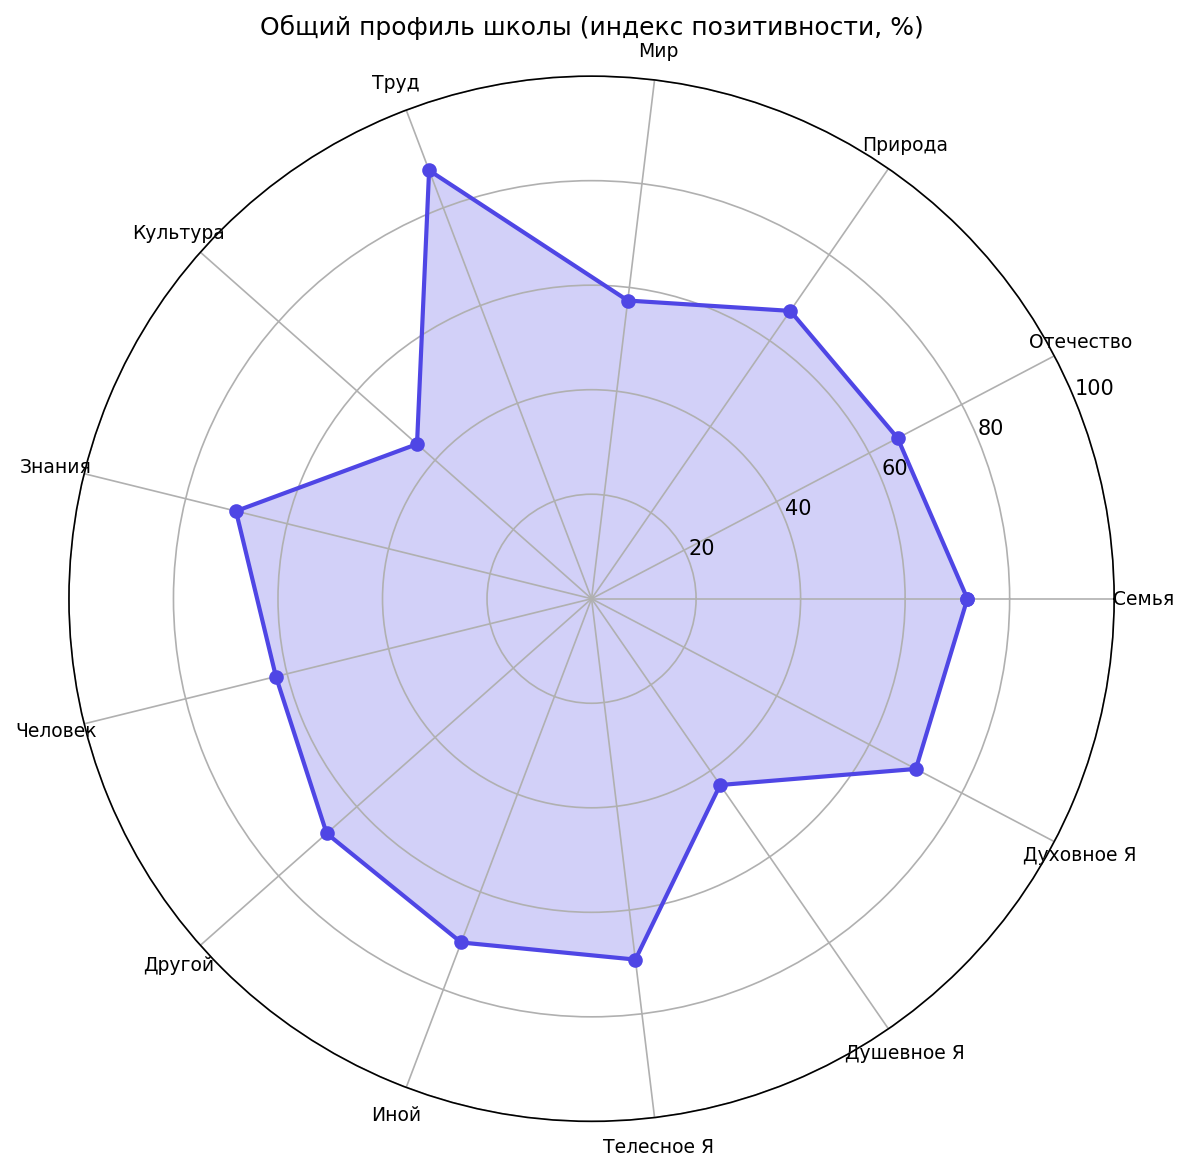
\includegraphics[width=0.72\textwidth]{figures/radar_school.png}
    \caption{Общий профиль школы (индекс позитивности по шкалам)}
    \label{fig:radar}
\end{figure}

\begin{figure}[H]
    \centering
    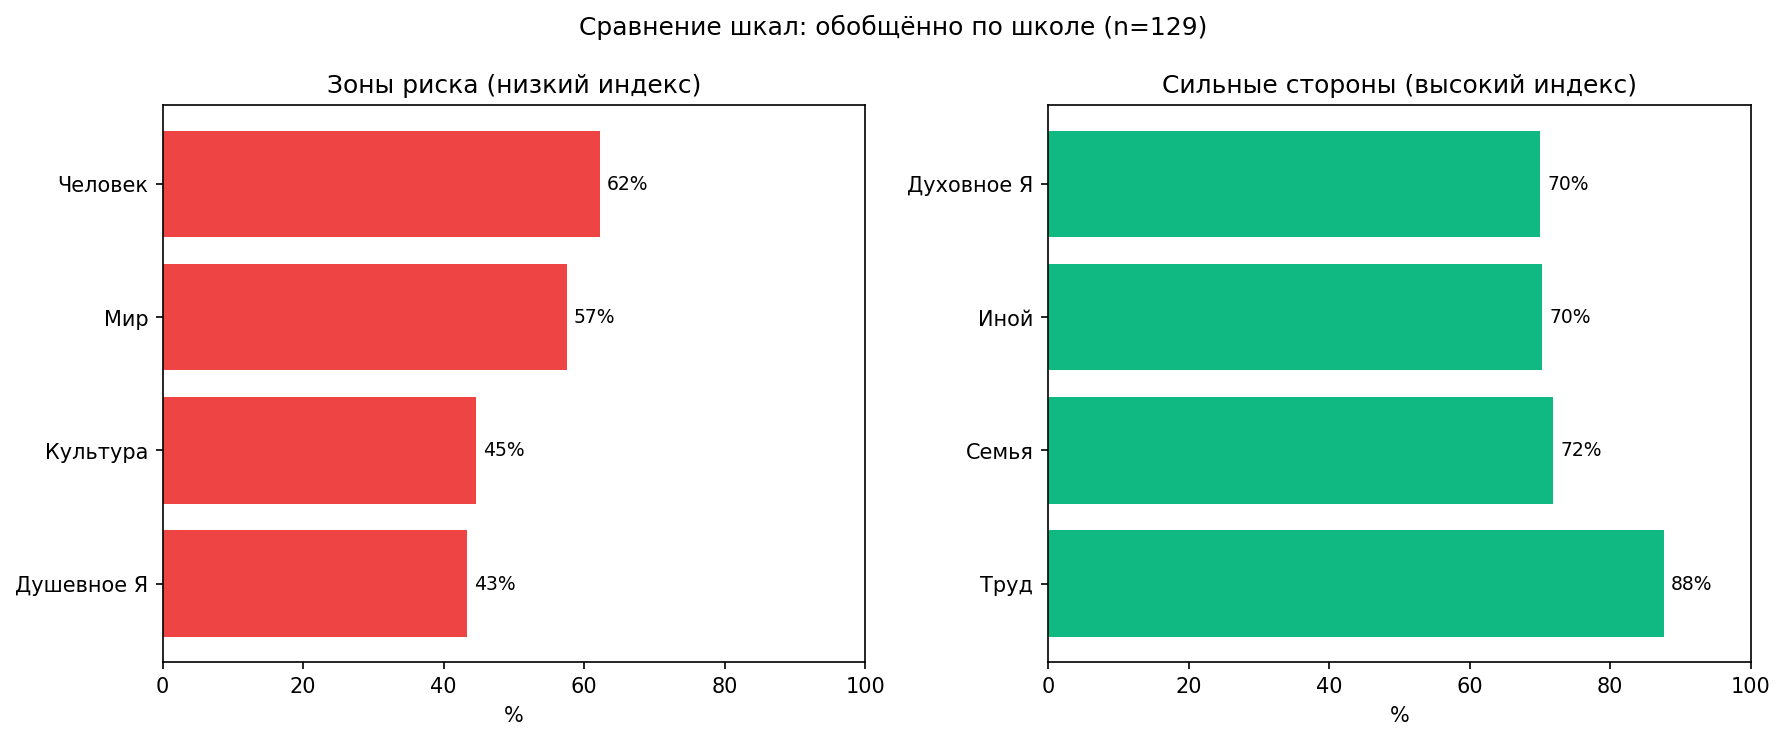
\includegraphics[width=\textwidth]{figures/strengths_risks.png}
    \caption{Сильные стороны и зоны риска (обобщённо, $n=127$)}
    \label{fig:sr}
\end{figure}

\subsection{Структура ответов по проблемным шкалам}

По шкале \textbf{«душевное Я»} (рис.~\ref{fig:soul}) доминируют ситуативный и устойчивый \textit{негатив} --- это признаки тревожности, неуверенности, эмоциональной нестабильности у значительной части учащихся.

По шкале \textbf{«культура»} (рис.~\ref{fig:cult}) --- преобладает ситуативный негатив: пренебрежительное отношение к культурным нормам, традициям, нравственным ориентирам в ряде ситуаций.

\begin{figure}[H]
    \centering
    \begin{minipage}{0.48\textwidth}
        \centering
        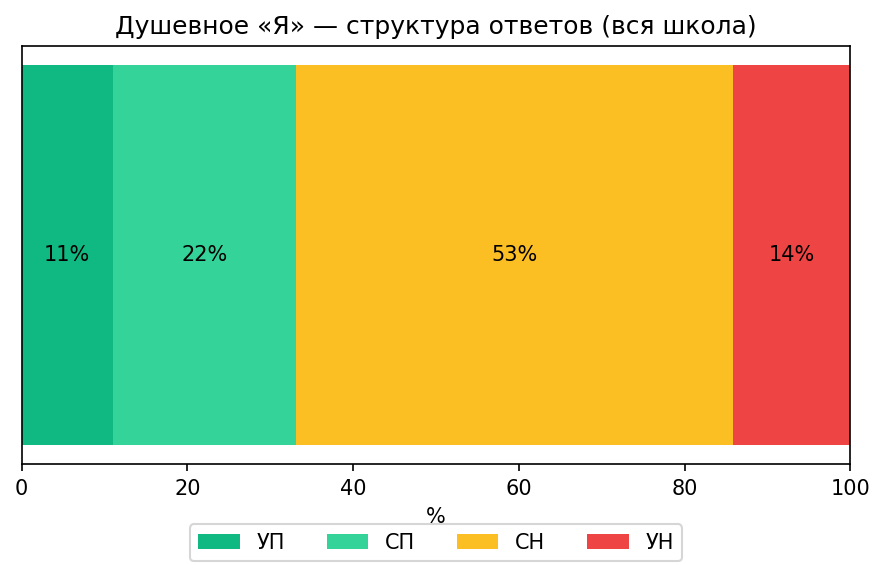
\includegraphics[width=\textwidth]{figures/stack_soul.png}
        \caption{Душевное «Я» (школа)}
        \label{fig:soul}
    \end{minipage}\hfill
    \begin{minipage}{0.48\textwidth}
        \centering
        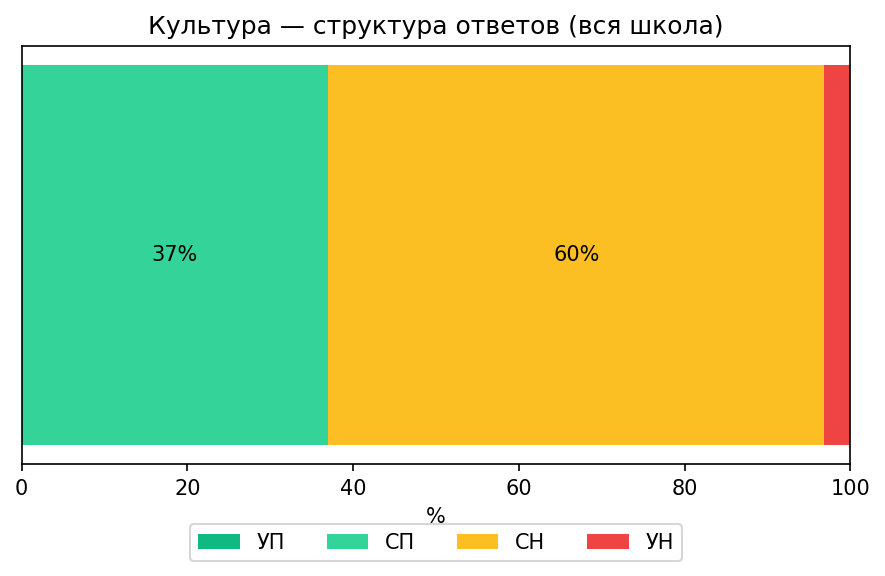
\includegraphics[width=\textwidth]{figures/stack_culture.png}
        \caption{Культура (школа)}
        \label{fig:cult}
    \end{minipage}
\end{figure}

\section{Ситуация по классам}

\subsection{Сводная таблица}

\small
\begin{center}
\begin{tabular}{@{}lrrrrr@{}}
\toprule
\textbf{Класс} & \textbf{$n$} & \textbf{Средний индекс} & \textbf{Труд} & \textbf{Культура} & \textbf{Душевное «Я»} \\
\midrule
10Б & 20 & 69\% & 100\% & 55\% & 35\% \\
10А & 18 & 64\% & 100\% & 33\% & 33\% \\
11А & 34 & 66\% & 100\% & 41\% & 35\% \\
9А  & 26 & 66\% & 96\%  & 35\% & 35\% \\
9Б  & 29 & 61\% & 93\%  & 24\% & 28\% \\
\midrule
\textbf{Школа} & \textbf{127} & \textbf{65\%} & \textbf{98\%} & \textbf{37\%} & \textbf{33\%} \\
\bottomrule
\end{tabular}
\end{center}
\normalsize

\subsection{Графики по классам}

На рис.~\ref{fig:heat} --- сравнение всех классов по 13~шкалам (чем зеленее ячейка, тем выше индекс). Видно, что \textbf{9Б} систематически «холоднее» по ряду шкал, особенно культура и душевное «Я».

\begin{figure}[H]
    \centering
    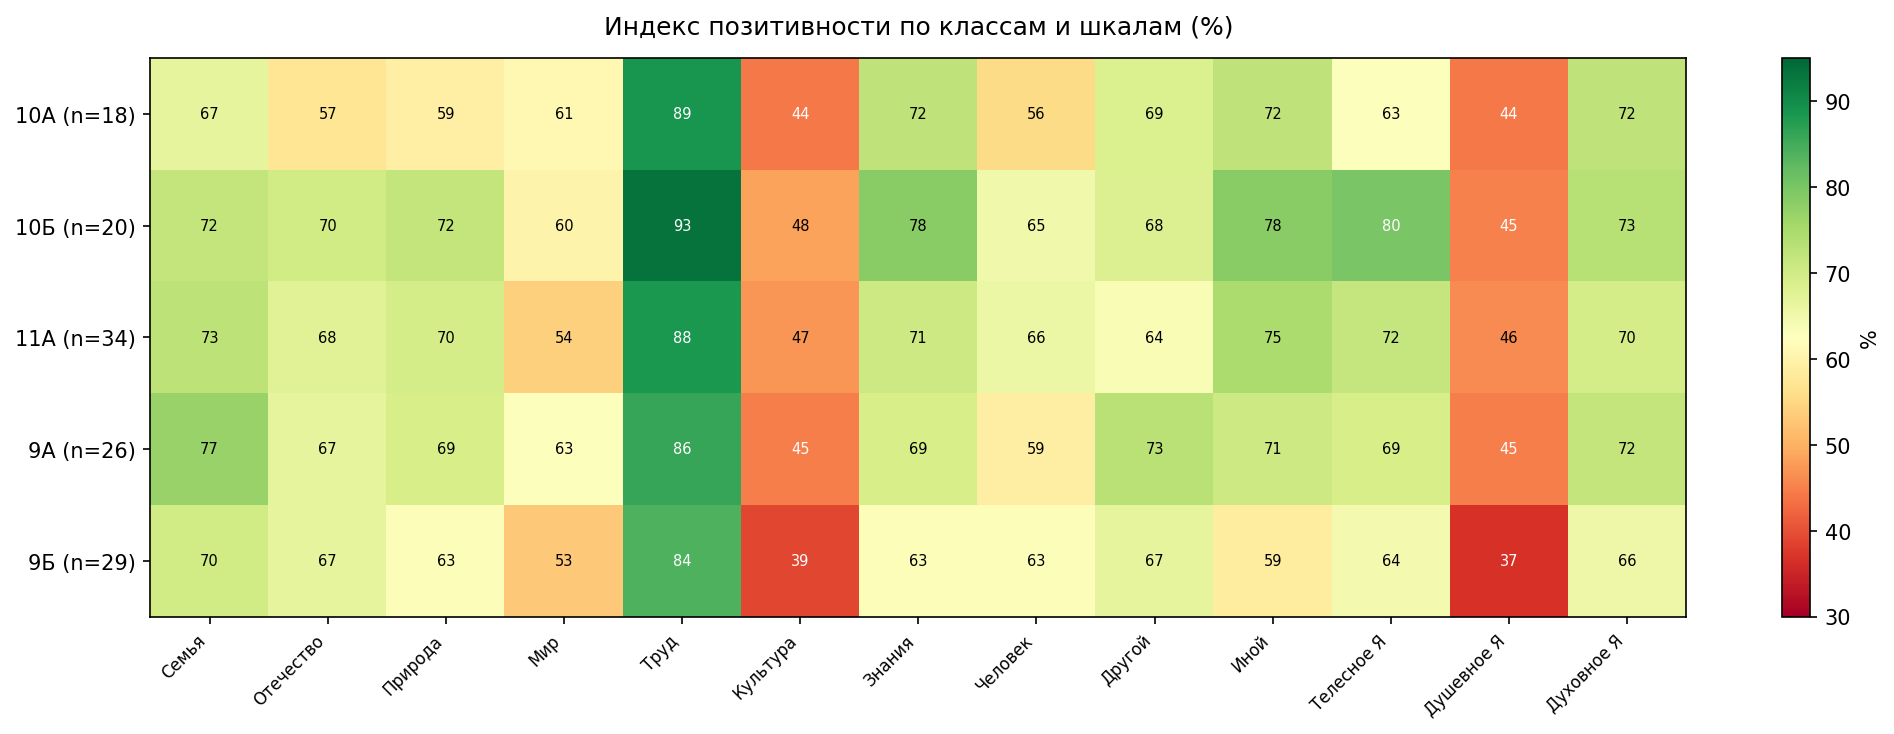
\includegraphics[width=\textwidth]{figures/heatmap_classes.png}
    \caption{Индекс позитивности: классы и шкалы}
    \label{fig:heat}
\end{figure}

\begin{figure}[H]
    \centering
    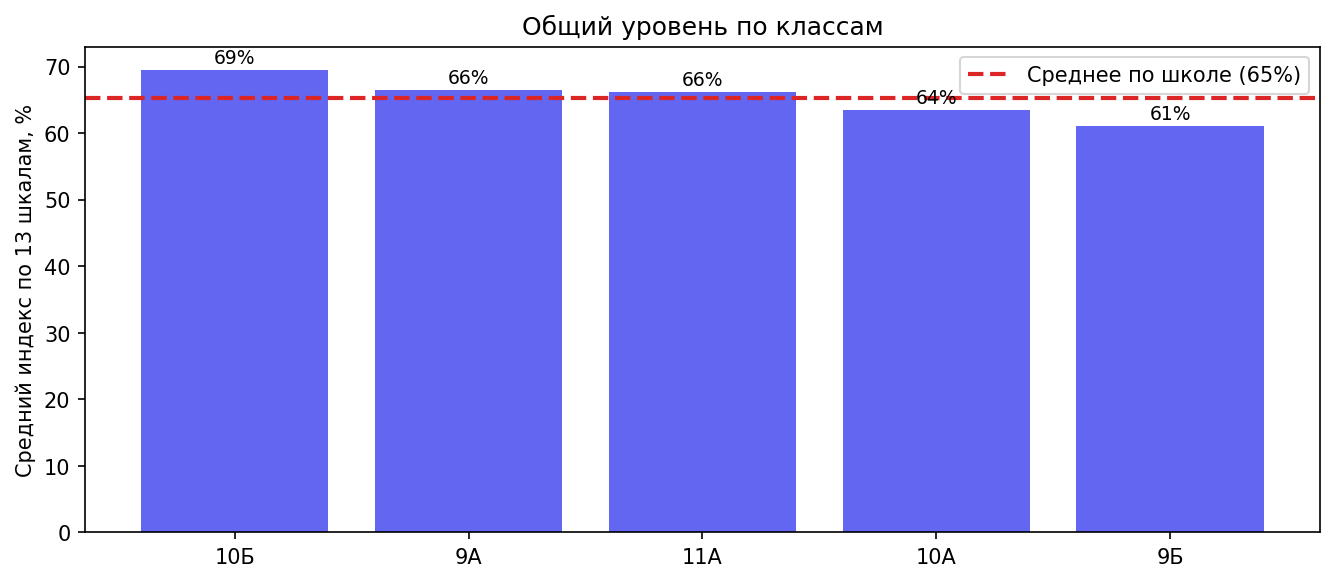
\includegraphics[width=0.92\textwidth]{figures/classes_overall.png}
    \caption{Средний индекс по классам (усреднение 13~шкал)}
    \label{fig:cls}
\end{figure}

\begin{figure}[H]
    \centering
    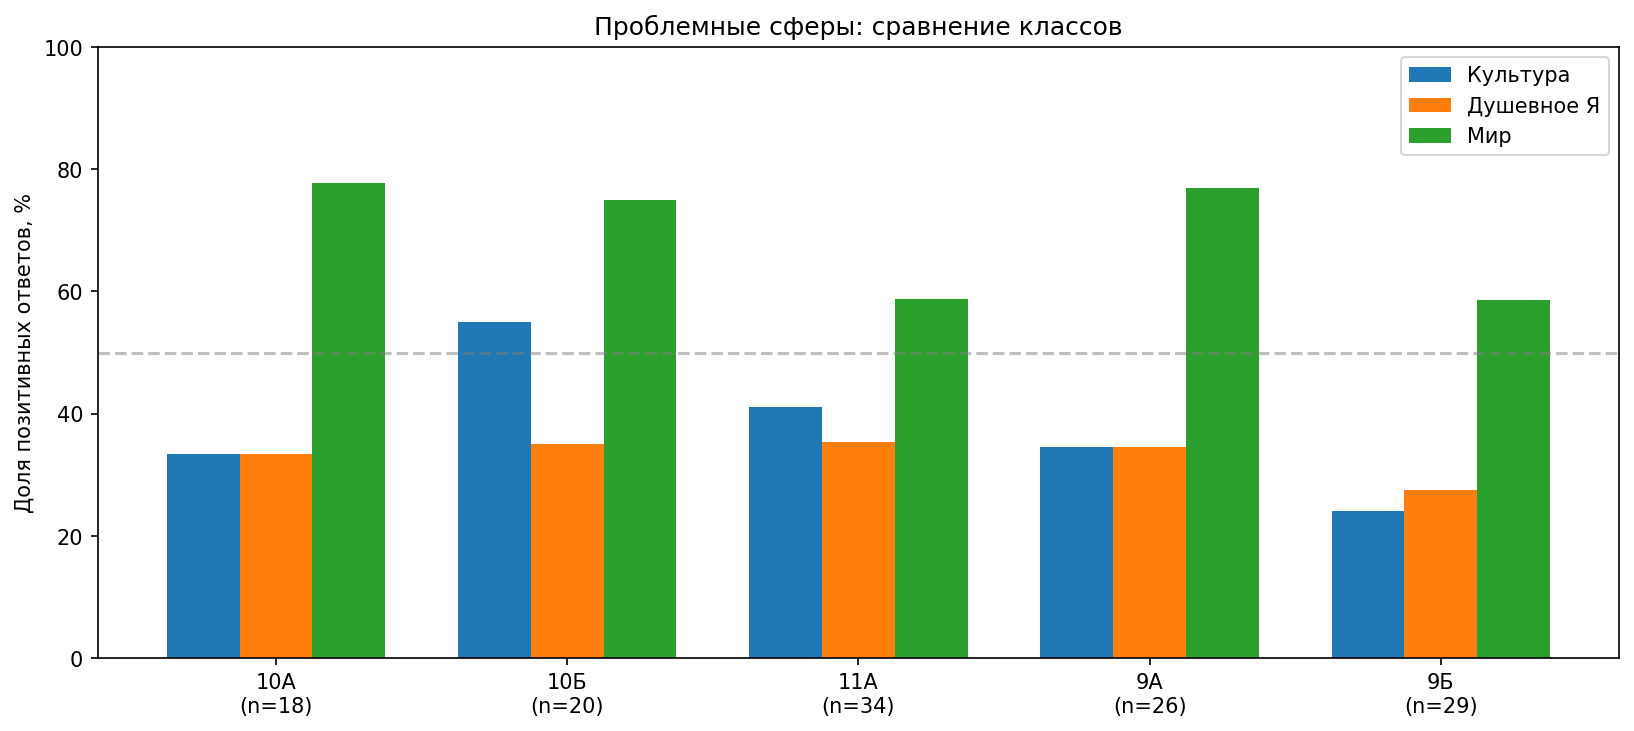
\includegraphics[width=\textwidth]{figures/classes_risk.png}
    \caption{Проблемные сферы: культура, душевное «Я», мир --- по классам}
    \label{fig:risk}
\end{figure}

\subsection{Краткая характеристика классов}

\textbf{10Б} ($n=20$) --- относительно благополучный класс: наивысший средний индекс (69\%), по культуре лучший показатель среди основных классов (55\%). Рекомендуется использовать как ресурсную группу для проектов наставничества.

\textbf{10А} ($n=18$) --- средний уровень; труд и учеба --- сильная сторона; культура и душевное «Я» --- по 33\% позитива, нужна профилактическая работа.

\textbf{11А} ($n=34$) --- крупнейшая выборка выпускного звена: стабильный средний уровень, труд --- 100\% позитива; культура и эмоциональная сфера --- зона внимания (около 35--41\%).

\textbf{9А} ($n=26$) --- средний профиль; умеренные риски по культуре и душевному «Я».

\textbf{9Б} ($n=29$) --- \textbf{приоритетный класс для поддержки}: наименьший средний индекс (61\%), культура --- 24\% позитива (наихудший показатель), душевное «Я» --- 28\%. Целесообразны беседы с классным руководителем, психологом, тематические классные часы.

\section{Рекомендации: на что обратить внимание и что усилить}

\subsection{Для всей школы}

\begin{enumerate}
    \item \textbf{Эмоциональное благополучие} --- ввести в план регулярные встречи с психологом, тренинги саморегуляции, профилактику тревожности (особенно 9--11~классы, предэкзаменационный период).
    \item \textbf{Культурное воспитание} --- экскурсии, встречи с носителями культуры, литературные и исторические проекты, обсуждение норм речи и поведения.
    \item \textbf{Закрепление ресурса} --- опираться на позитив к труду и знаниям: проекты, волонтёрство, наставничество старших классов.
    \item \textbf{Гражданско-нравственное воспитание} --- дискуссии о толерантности, уважении к «Другому» и «Иному», развитие диалога без крайних оценок.
\end{enumerate}

\subsection{По классам (приоритеты)}

\begin{itemize}
    \item \textbf{9Б} --- первоочередно: психологическая поддержка + культурно-просветительский блок; контроль эмоционального климата в коллективе.
    \item \textbf{9А, 10А, 11А} --- профилактика по культуре и душевному «Я»; для 11А --- поддержка выпускников.
    \item \textbf{10Б} --- закрепление успешного опыта; вовлечение в лидерские и наставнические роли.
\end{itemize}

\subsection{Работа с родителями}

Информировать о \textit{общих} результатах (без персональных данных), давать рекомендации: поддержка ребёнка дома, внимание к эмоциональному состоянию, совместные культурные мероприятия.

\small
\begin{longtable}{@{}p{3.8cm}p{10.5cm}@{}}
\toprule
\textbf{Направление} & \textbf{Примеры мероприятий} \\
\midrule
\endhead
Психолог & Консультации; «Как справляться со стрессом»; профилактика перед ОГЭ/ЕГЭ \\
Культура & Музеи, театры; неделя культуры; дискуссии о традициях \\
Нравственность & Волонтёрство; взаимопомощь в классе \\
Патриотизм & Встречи с ветеранами; проекты о малой родине \\
Семья & Родительские собрания с обобщёнными результатами \\
\bottomrule
\end{longtable}
\normalsize

\section{Заключение}

Диагностика показала: в школе сформирован \textbf{сильный ресурс} в сфере труда, учёбы, семьи и природы. Одновременно выявлены \textbf{системные риски} в эмоциональной сфере (душевное «Я») и культуре --- особенно в 9Б, 9А и 10А. Рекомендуется включить в план воспитательной работы целевые меры поддержки и использовать интерактивный отчёт для мониторинга по классам.

\vspace{1em}
\noindent\small\textit{Справка подготовлена по данным опроса. Графики: настоящий документ и \url{https://misaicpacmak.github.io/survey-report/}}

\end{document}
